\begin{figure}[!htb]
\setlength{\unitlength}{\textwidth}

  \begin{picture}(1,0.38)(0,0.74)
    
  \put(0.4,0.76){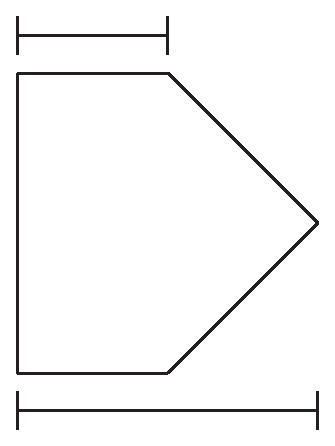
\includegraphics[width=0.25\unitlength]{./chapter-cross-sections/fnp/hybrid_section.eps}}         
      
      
   
 	\put(0.46,1.095){$d$}
 	\put(0.52,0.74){$l$}
   \

 	
 	 

     

  \end{picture}

 \caption{Illustration of the hybrid cross section (combination of a square and a triangle) obtained by tapering the afterbody of the square. The afterbody was changed by changing the ratio of $\ratio$. Hence, data were obtained for $\ratio=1, 0.75, 0.5, 0.25$\ and $0$ were considered in this study.}
    \label{fig:hybrid_section}
\end{figure}